\makeatletter
\def\input@path{{../Distributed-and-Pervasive-Systems/}}
\makeatother
\documentclass[a4paper,10pt,oneside]{memoir}
% Dokumentklassen sættes til memoir.
% Manual: http://ctan.org/tex-archive/macros/latex/contrib/memoir/memman.pdf
%\documentclass[a4paper,11pt,twoside,openright]{memoir}
\setlrmarginsandblock{*}{2.5cm}{0.75} % højre og venstre 
\setulmarginsandblock{3cm}{*}{1.2} % top og bund 
\checkandfixthelayout[nearest] % specifikt valg af højde algoritme

%Styrer hvordan nye afsnit håndteres
%https://www.sharelatex.com/learn/Paragraph_formatting#Reference_guide
\parindent=1em %Start på nyt afsnit rykkes ind
\parskip=0.5em %Mellemrum mellem afsnit
 
% Danske udtryk (fx  og tabel) samt dansk orddeling og fonte med
% danske tegn. Hvis LaTeX brokker sig over æ, ø og å skal du udskifte
% "utf8" med "latin1" eller "applemac". 
\usepackage[utf8]{inputenc}
\usepackage[english]{babel}
\usepackage[T1]{fontenc}
\usepackage{mflogo}
\usepackage{titlesec}
\titleformat{\chapter}[hang] 
{\normalfont\huge\bfseries}{\chaptertitlename\ \thechapter:}{1em}{} 
\titlespacing*{\chapter}{0pt}{-50pt}{40pt}

%bruges til at fastgøre billeder hvor man vil have dem ved brug af H
\usepackage{float}

%sexy pdf'er
%\usepackage[export]{adjustbox}
\usepackage{pdfpages}
\usepackage{pdflscape}

%Kompakte lister
\usepackage{paralist}
 
% Matematisk udtryk, fede symboler, theoremer og fancy ting (fx kædebrøker)
\usepackage{amsmath,amssymb}
\usepackage{bm}
\usepackage{amsthm}
\usepackage{mathtools}

% Fancy ting med enheder og datatabeller. Læs manualen til pakken
% Manual: http://www.ctan.org/tex-archive/macros/latex/contrib/siunitx/siunitx.pdf
\usepackage{siunitx}
 
%Fancy headers, 
%Manual: https://www.sharelatex.com/learn/Headers_and_footers
\let\footruleskip\undefined
\usepackage{fancyhdr}
\pagestyle{fancy}

 
% Indsættelse af grafik. og man kan rotere tekst in line
\usepackage{graphicx} 
\usepackage{fix-cm} 
\usepackage{soul}
\sodef\an{}{0.13em}{0em}{0em} \sodef\ann{}{0.13em}{0.5em}{0em}
 

%Fancy tabeller.
%\usepackage[table]{xcolor}
\usepackage{multirow}
\usepackage{rotating} %sidewaystables!
\usepackage{longtable} %tables spanning multible pages.
\usepackage{tablefootnote} %for at indstætte fornoter i tabeller.
\usepackage{hhline} %Fixer farvede felter
\usepackage{ltxtable} %Longtabular X
\usepackage{tabularx} %Med dynamisk bredte

%URL fodnoter
\usepackage{url}

% Reaktionsskemaer. Læs manualen for at se eksempler.
% Manual: http://www.ctan.org/tex-archive/macros/latex/contrib/mhchem/mhchem.pdf
\usepackage[version=3]{mhchem}

%Lav chapter clickable og fjern border
\usepackage{hyperref}
\hypersetup{
    colorlinks,
    citecolor=black,
    filecolor=black,
    linkcolor=black,
    urlcolor=black
}

%Table of contents settings
\setsecnumdepth{subsection} % organisational level that receives a numbers
\settocdepth{subsection}   % print table of  for level 3

%Til programkode
\usepackage{listings}
\usepackage{color}

\definecolor{dkgreen}{rgb}{0,0.6,0}
\definecolor{gray}{rgb}{0.5,0.5,0.5}
\definecolor{mauve}{rgb}{0.58,0,0.82}
 
\lstset{ 
  language=C++,                % the language of the code
  basicstyle=\footnotesize,           % the size of the fonts that are used for the code
  numbers=left,                   % where to put the line-numbers
  numberstyle=\tiny\color{gray},  % the style that is used for the line-numbers
  stepnumber=1,                   % the step between two line-numbers. If it's 1, each line 
                                  % will be numbered
  numbersep=5pt,                  % how far the line-numbers are from the code
  backgroundcolor=\color{white},      % choose the background color. You must add \usepackage{color}
  showspaces=false,               % show spaces adding particular underscores
  showstringspaces=false,         % underline spaces within strings
  showtabs=false,                 % show tabs within strings adding particular underscores
  frame=single,                   % adds a frame around the code
  rulecolor=\color{black},        % if not set, the frame-color may be changed on line-breaks within not-black text (e.g. commens (green here))
  tabsize=2,                      % sets default tabsize to 2 spaces
  captionpos=b,                   % sets the caption-position to bottom
  breaklines=true,                % sets automatic line breaking
  breakatwhitespace=false,        % sets if automatic breaks should only happen at whitespace
  title=\lstname,                   % show the filename of files included with \lstinputlisting;
                                  % also try caption instead of title
  keywordstyle=\color{blue},          % keyword style
  commentstyle=\color{dkgreen},       % comment style
  stringstyle=\color{mauve},         % string literal style
  escapeinside={\%*}{*)},            % if you want to add LaTeX within your code
  morekeywords={*,...},               % if you want to add more keywords to the set
  rangeprefix=//----------,			%Used for sexy code includes
  rangesuffix=----------,			%---||---
  includerangemarker=false,			%---||---
  literate=
  {á}{{\'a}}1 {é}{{\'e}}1 {í}{{\'i}}1 {ó}{{\'o}}1 {ú}{{\'u}}1
  {Á}{{\'A}}1 {É}{{\'E}}1 {Í}{{\'I}}1 {Ó}{{\'O}}1 {Ú}{{\'U}}1
  {à}{{\`a}}1 {è}{{\`e}}1 {ì}{{\`i}}1 {ò}{{\`o}}1 {ù}{{\`u}}1
  {À}{{\`A}}1 {È}{{\'E}}1 {Ì}{{\`I}}1 {Ò}{{\`O}}1 {Ù}{{\`U}}1
  {ä}{{\"a}}1 {ë}{{\"e}}1 {ï}{{\"i}}1 {ö}{{\"o}}1 {ü}{{\"u}}1
  {Ä}{{\"A}}1 {Ë}{{\"E}}1 {Ï}{{\"I}}1 {Ö}{{\"O}}1 {Ü}{{\"U}}1
  {â}{{\^a}}1 {ê}{{\^e}}1 {î}{{\^i}}1 {ô}{{\^o}}1 {û}{{\^u}}1
  {Â}{{\^A}}1 {Ê}{{\^E}}1 {Î}{{\^I}}1 {Ô}{{\^O}}1 {Û}{{\^U}}1
  {œ}{{\oe}}1 {Œ}{{\OE}}1 {æ}{{\ae}}1 {Æ}{{\AE}}1 {ß}{{\ss}}1
  {ç}{{\c c}}1 {Ç}{{\c C}}1 {ø}{{\o}}1 {å}{{\r a}}1 {Å}{{\r A}}1
  {€}{{\EUR}}1 {£}{{\pounds}}1
}

%Til at udregne forskel mellem sider, brug \pagedifference{A}{B} mellem to labels A og B.
\usepackage{refcount}
\newcommand{\pagedifference}[2]{%
  \number\numexpr\getpagerefnumber{#2}-\getpagerefnumber{#1}\relax}
 
%Til at lave referencer med:
\usepackage{cite}

%Til at lave eksterne \ref til \labels
\usepackage{xr}

%Til at lave \Beam (DC symbol)
\usepackage{marvosym}

%Forsøg på nice lister i tabeller
\usepackage[shortlabels]{enumitem}

\newenvironment{packed_enum}{
\begin{enumerate}[1., topsep=0pt, nosep, partopsep=0pt, itemsep=0pt, parsep=0pt]
}{\end{enumerate}}

\newenvironment{packed_item}{
\begin{itemize}[•, topsep=0pt, nosep, partopsep=0pt, itemsep=0pt, parsep=0pt]
}{\end{itemize}}

%Lækker kommando til at skrive I2C flot uden at bruge \textsuperscript hver gang:
\newcommand*{\IIC}{\texorpdfstring{I\textsuperscript{2}C }{I2C}}

%Lækker kommando til ref. -> \ref{input} \nameref{input} på side \pageref{input}
\newcommand*{\myRef}[1] {\ref{#1} \nameref{#1} på side \pageref{#1}}

%Lorem ipsum
\usepackage{lipsum}


\usepackage{longtable}
\usepackage{array} % for extrarowheight

%Juicy columntypes - http://tex.stackexchange.com/questions/12703/how-to-create-fixed-width-table-columns-with-text-raggedright-centered-raggedlef
\newcolumntype{L}[1]{>{\raggedright\let\newline\\\arraybackslash\hspace{0pt}}p{#1}}
\newcolumntype{C}[1]{>{\centering\let\newline\\\arraybackslash\hspace{0pt}}p{#1}}
\newcolumntype{R}[1]{>{\raggedleft\let\newline\\\arraybackslash\hspace{0pt}}p{#1}}
\newcolumntype{Z}{>{\raggedright\arraybackslash}X}

%Dejlig kommando til at få nye kapitler på højre side
\newcommand*\cleartorightpage{%
	\clearpage
 	\checkoddpage
	\ifoddpage
  		%do nothing
	\else
		\thispagestyle{empty}
		\mbox{}
 		\clearpage
	\fi
}


%Hacky løsning til at ordne indholdsfortegnelsen.. Why memoir class.. WHY??!
\renewcommand*{\cftdotsep}{1}
\setpnumwidth{3em}
\setrmarg{4em}

%Bugfix til Longtables
\makeatletter
\def\LT@start{%
  \let\LT@start\endgraf
  \endgraf\penalty\z@\vskip\LTpre
  \dimen@\pagetotal
  \advance\dimen@ \ht\ifvoid\LT@firsthead\LT@head\else\LT@firsthead\fi
  \advance\dimen@ \dp\ifvoid\LT@firsthead\LT@head\else\LT@firsthead\fi
  \advance\dimen@ \ht\LT@foot
  \edef\restore@vbadness{\vbadness\the\vbadness\relax}% (added)
  \vbadness=\@M % (added)
  \dimen@ii\vfuzz
  \vfuzz\maxdimen
    \setbox\tw@\copy\z@
    \setbox\tw@\vsplit\tw@ to \ht\@arstrutbox
    \setbox\tw@\vbox{\unvbox\tw@}%
  \vfuzz\dimen@ii
  \restore@vbadness % (added)
  \advance\dimen@ \ht
        \ifdim\ht\@arstrutbox>\ht\tw@\@arstrutbox\else\tw@\fi
  \advance\dimen@\dp
        \ifdim\dp\@arstrutbox>\dp\tw@\@arstrutbox\else\tw@\fi
  \advance\dimen@ -\pagegoal
  \ifdim \dimen@>\z@\vfil\break\fi
      \global\@colroom\@colht
  \ifvoid\LT@foot\else
    \advance\vsize-\ht\LT@foot
    \global\advance\@colroom-\ht\LT@foot
    \dimen@\pagegoal\advance\dimen@-\ht\LT@foot\pagegoal\dimen@
    \maxdepth\z@
  \fi
  \ifvoid\LT@firsthead\copy\LT@head\else\box\LT@firsthead\fi\nobreak
  \output{\LT@output}%
}
\makeatother

%Debugging
%\overfullrule=2cm
\usepackage{amsmath}
\usepackage{amsfonts}
\usepackage{amssymb}
\title{Distributed and Pervasive Systems \\ Team 2}
\author{Report \\ Aarhus University, Science and Technology \\ Lector: Christian Fischer Pedersen}
\date{\today}
\begin{document}
\fancyhf{} %Clear all header/footers
\frontmatter
\maketitle
\vfill

%\begin{figure}
%	\centering
%	\includegraphics[scale=1, trim=125 110 120 650, clip=true]{../fig/forside_rapport_underskrevet}
%\end{figure}

\begin{table} [h]
	\centering
	\begin{tabular}{|l|r|}
	\hline 
	\textbf{Name} 				& \textbf{Study number}	\\ \hline
	David Jensen 				& 11229 	  			\\ \hline
	Henrik Bagger Jensen 		& 201304157  			\\ \hline
	Ólafur Dagur Skúlason 		& IY11249	 			\\ \hline
	Titas Urbonas 				& 201700321  			\\ \hline
	Christian Lillelund 		& 201408354 			\\ \hline

	\end{tabular}
\end{table}

\vfill

\clearpage
\pagestyle{plain}

\tableofcontents

\vfill

\mainmatter
\pagestyle{fancy}
\fancyhf{} %Clear all header/footers
\fancyhead[RO,LE]{Team 2 - Report}
\fancyhead[CE,CO]{\nouppercase{\leftmark}}
\fancyhead[LO,RE]{Aarhus University}
\fancyfoot[CO,CE]{\nouppercase{\rightmark}}
\fancyfoot[LE,RO]{\thepage}

\chapter{Introduction} \label{ch:introduction}

In recent years we have seen an increase in the number of systems being split up and distributed, as the need of offloading the workload from a single computing entity to multiple has grown. From the first mechanical computers in the late 40's, past Apple's Macintosh in 1984 and when the first smartphones start appearing in the 2000's, to the era of modern cloud computing, we have seen a shift from centralized and single processor computing to distributed with multiple processors involved. This is due to a few aspects: The costs of hardware and power requirements have gone down (Koomey's law)\footnote{\cite{Koomey2011}}, making it more feasibly to link multiple computers instead of buying one large. Modern systems require a high degree of fault tolerance, which distributing a system can assist with. Also it opens up for improved concurrency and parallelism when you can allocate computing tasks to multiple node, facilitated by the fact that the storage capabilities of computers are increasing too (Kryder's law)\footnote{\cite{Walter2005}}.

Along with distributed computing comes pervasive systems - to have computers and technology appear anytime and everywhere require to some extent a distributed system. The smart home, for example, has multiple nodes and sensors placed indoors to detect movement, hear voice commands and relay instructions often to bigger and more complex systems. When the owner is asking for something, the system must decipher: Who is asking? What is he asking about? Where is he right now? This requires interoperability and multiple processors to work together.

Computers are getting more powerful every day (Moore's law)\footnote{\cite{Moore1965}} and now becoming more distributed than we have seen before. In this project we will explore important concepts of distributed systems, some of the methods and algorithms used and how various applications built on top of a distributed network topology.				\clearpage
\chapter{Real-Time Computing} \label{ch:realTimeComputing}

%-- C(l)ock Synchronization? hue hue

\section{Determinism} \label{sc:determinism}

- Finite automata for determined/undetermined systems
Short intro, an example\\
DFA\\
NFA\\
TFA\\
Compare deterministic and non-deterministic automata
Talk about timed automatas and how they comply with deadlines

\section{Scheduling} \label{sc:scheduling}
In scheduling the aim is to meet all hard deadlines and handle soft deadlines of jobs in the best possible manner and avoid deadlocks while doing so. The arrival time of a job is the moment in time it arrives at a processor, while the release time of a job is the moment in time it becomes available for execution. A task can have different job types and such as periodic, sporadic and aperiodic. A task is a set of jobs known at the start of the system or triggered by a external event.

A periodic task is defined by three parameters:
\begin{itemize}
	\itemsep0em
	\item The release time \textit{r} of the first periodic job.
	\item The period \textit{p}, which is a periodic time interval, at the start of which a periodic job is released.
	\item The execution time \textit{e} of each periodic job.
	\item The deadline \textit{d} of each periodic job.
\end{itemize}
and is written as $J_n=(r,p,e,d$)

\subsection{Rate-monotonic scheduler}
The rate-monotonic scheduling strategy gives a higher priority to periodic jobs with a shorter period. Because of the static nature of the scheduler, it is easy to compute and predict.\footnote{\cite[p.~183]{Fokkink1965}}
%--- This can be removed if we need space?
We define three periodic jobs: $J_1$ with a period of 20 and a execution time of 3, $J_2$ with a period of 5 and a execution time of 2, $J_3$ with a period of 10 and a execution time of 2. All with a release time of 0. Figure \ref{fig:rateMonotonicExample} shows the execution of the three jobs using a rate-monotonic scheduler.
%---

\begin{figure}[!h]
	\centering
	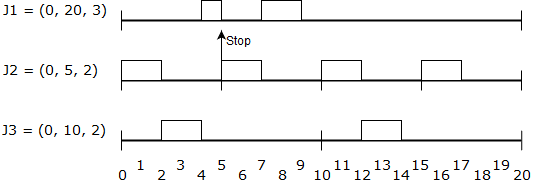
\includegraphics[scale=0.5]{realTimeComputing/fig/rate-mono.png}
	\caption{Example of rate-monotonic scheduling.}
	\label{fig:rateMonotonicExample}
\end{figure}

As can be seen on Figure \ref{fig:rateMonotonicExample}, the first job to be executed is $J_2$ followed by $J_3$. $J_1$ is then started but gets preempted by the scheduler, because $J_2$ starts a new execution on period 5. $J_2$ has a shorter period and therefore has a higher priority. $J_3$ continues execution after $J_1$.

\subsection{Earliest deadline first scheduler}
This scheduling strategy will give a higher priority to jobs if their deadline is
early. In case of preemptive jobs and no competition for resources, this scheduler
is optimal, in the sense that if utilization at a processor does not exceed one, then
periodic jobs will be scheduled in such a way that no deadlines are missed.\footnote{\cite[p.~184]{Fokkink1965}}

\begin{figure}[!h]
	\centering
	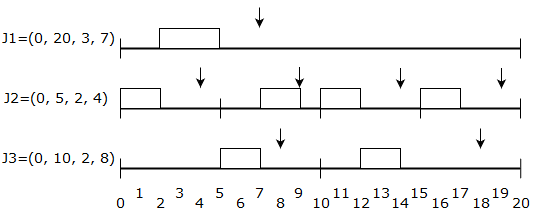
\includegraphics[scale=0.5]{realTimeComputing/fig/EarliestDeadlineFirst.png}
	\caption{Example of Earliest deadline first or Least-slacktime-first scheduler.}
	\label{fig:EarliestDeadlineFirstAndLeastSlacktimeFirstSchedulerExample}
\end{figure}

The example in Figure \ref{fig:EarliestDeadlineFirstAndLeastSlacktimeFirstSchedulerExample} can be viewed as using Earliest deadline first scheduler. This approach is dynamic meaning it evaluates the jobs each time unit. The first job to be executed is $J_2$ because it has earliest deadline followed by $J_1$ and $J_3$.

\subsection{Least-slacktime-first scheduler}
This scheduling strategy gives higher priority to jobs with less slack time (i.e. idle time). This scheduler is a good choice if utilization at a processor does not exceed one. In this case the periodic jobs will be scheduled in such a way that no deadlines are missed.\footnote{\cite[p.~184]{Fokkink1965}} We use the following formula to determine the slacktime: $L(T)=D(T)-C(T)$, Where $T$ represent the time, $L(T)$ represent the laxity (slack), $D(T)$ represent the time between the closest deadline and the current time, $C(T)$ represent the remaining time of execution. For each time-frame a calculation of all the processes are done and the one with the least slacktime will be prioritized.

The example in Figure \ref{fig:EarliestDeadlineFirstAndLeastSlacktimeFirstSchedulerExample} can be viewed as using Least-slack time-first scheduler. Note that it is a coincidence that both least-slacktime-first and deadline first schedulers act the same, for this example. At $T=0$ the three formulas will look as follows:
\begin{align}
	L_1(0)=7-3&=4 \\
	L_2(0)=4-2&=2 \\
	L_3(0)=8-2&=6
\end{align}
At $T=0$, $J_2$ has the least slack and is therefore prioritized. This procedure will be followed for every timeframe and the job with least slack will be prioritized. In case the slack of two jobs are the same (As at time $T=4$ and $T=6$, in this example), the process that is currently running will be prioritized.

\section{Resource control}

One of the pitfalls of sharing resources is deadlocks, as competing processes wanting the same resource could introduce race conditions\footnote{Race conditions: A race condition or race hazard is the behavior of an electronics, software, or other system where the output is dependent on the sequence or timing of other uncontrollable events.} resulting in the jobs blocking each other and often an unpredictable outcome. We consider a high priority Task H, a medium priority task M and a low priority Task L. When a phenomenon called priority inversion occurs, Task H is preempted by a lower priority task, causing the priorities to be inverted. This could occur if Task L is using some shared resource R in its critical section, Task H arrives requesting R, but gets blocked because it is in use by Task L. Now a Task M starts executing during Task L's use of R, and since Task H is blocked waiting for Task L, Task M is now the highest priority task in the system, so it occupies the processor without nobody being able to preempt it. Task H is now at the bottom of the executing chain waiting for Task L that waits for Task M to finish. We will discuss two protocols that can remedy these issues named \textit{priority inheritance} and \textit{priority ceiling}.

\subsection{Priority inheritance}

This protocol uses dynamic priority adjustments to change task priorities on the fly. Assume Task L is running and uses some shared resource. If Task H arrives and requests ownership of the same shared resource, Task L gets elevated to the priority of the requesting Task H. Task L would then continue executing its critical section. Once it is done, the task gets dropped down to its original priority, allowing Task H to take control of the resource. Priority inheritance makes it less likely that a high priority job gets blocked by the lower one, however each nested resource lock would increase the wait time for a pending task to complete. The maximum wait time would be the sum of all the execution times of all of the nested resource locks.

\subsection{Priority ceiling}

With priority ceiling all tasks that will access a given shared resource are evaluated before executing and each resource is assigned a predefined priority based on the task with the highest priority that will access the resource. This is called a priority ceiling. When a task requires a resource, the task's priority is elevated to match that of the resource, ensuring that the task will not be preempted by any other task. Once it completes, the task is dropped down to its original priority. The maximum wait time for a high-priority task is limited to the longest critical section of any lower-priority task that accesses the shared resource.

	\clearpage
\chapter{Synchronization} \label{ch:synchronization}

\section{Logical Clock}\label{sc:logicalClock}

In an absence of real clocks, a logical clock would be applicable to coordinate task and allow ordering of events between nodes in a distributed system. Logical clocks range from mere counters, that periodically increments some integer value, to complex vector time stamps with multiple sets of integer vectors. In this section we look at the need for logical clocks, define a happened-before relation and Lamport scalar time stamps. Time is defined in terms different from \textit{t(x)}

\subsection{A framework for logical clocks}

We define the logical clock as \textit{C} consisting of a time domain \textit{T}. Relation \textit{->} is called the happened-before relation or earlier-than. The logical clock C maps an event e to a element in the time domain T, which we denote as C(e) and define as:

\[ C: E \longmapsto T \]
which satisfies the three properties for the happened-before relation:

\begin{itemize}
	\item Clock consistency: For two events $e_i$ and $e_j$, $e_i$ -> $e_j$ $\Longrightarrow$ C($e_i$) < C($e_j$)
	\item Contrapositive: If C($e_i$) $\nless$ C($e_j$), then $e_i$ $\nrightarrow$ $e_j$
	\item Strong consistency: $e_i$ -> $e_j$ $\Leftrightarrow$ C($e_i$) < C($e_j$)
\end{itemize}

To implement a logical clock in a system of multiple processes, we need to address two issues: A local data structure in each process $p_i$ to represent logical time and a protocol to update the data structures of other processes to ensure the clock consistency condition. This protocol ensures that process $p_j$ local clock and its view on the global clock is consistent, and can be implemented with Lamport time stamps. 

\subsection{Lamport time-stamps}

Invented by Leslie Lamport in 1978, it is an algorithm to order events in a system by using scalar time, a simple non-negative integer $C_i$ time stamp that each process in a system manages. To implement it, we look at at send-scenario, where $p_i$ relays a message to $p_j$.

\begin{itemize}
	\item Before a send event, process $p_i$ executes the following: $C_i$ $\colon$=  $C_i$ + d, where d is a non-zero scalar.
	\item Process $p_i$ sends the message to process $p_j$ containing a payload and the time stamp $C_i$.
	\item Process $p_j$ receives the message with time stamp $C_i$ and executes: $C_j$ $\colon$= max($C_j$,$C_i$) 
\end{itemize}

This ensures that process $p_j$ will update its local logical clock newest global logical clock whenever it receives messages from other processes, allowing events to happen at a more consistent basis now that a given process uses the most up-to-date global clock to know when to fire.

In Figure \ref{fig:lamport}, an example of three processes are given, with the lamport timestamp implementation.


\begin{figure}[H]
	\centering
	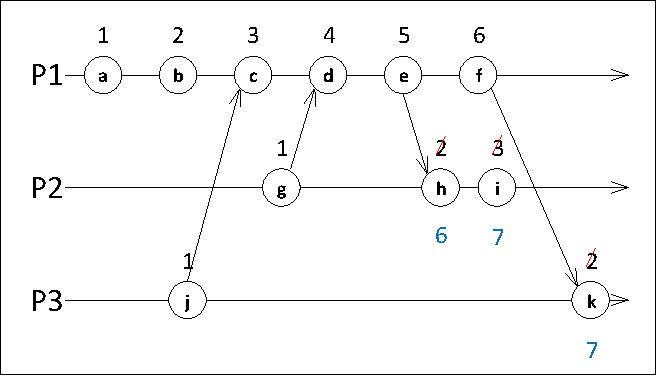
\includegraphics[width=0.3\linewidth]{synchronization/logicalClock/fig/lamport.pdf}
	\caption{An example of the lamport timestamp correction, with three processes \textit{P1}, \textit{P2} and \textit{P3}. Blue numbers are the correction of the lamport timestamps, since $e \rightarrow h$ and $f \rightarrow k$ both were in wrong order.}
	\label{fig:lamport}
\end{figure}


\section{Real Clock}\label{sc:realClock}

The real clocks are integrated circuit in electronics with the alternate power source for counting time when the electronics is off, which are used in the systems that needs to keep accurate time. Most of the systems uses crystal oscillator. Because of the clock drift there is a need to synchronize clocks. The two most used algorithms for it is PTP(Precision Time Protocol) and NTP(Network time Protocol) will be described separately below.

\subsection{The need for real clocks}

Why do we need real clocks? Can't we just use the logical ones u just talked about?
Some system needs to know real time(e.g. stock market, bank systems). Logical clocks wont work in this case, because we need precise time oftransactions.
Some system needs to know real time(e.g. stock market, bank systems). Logical clocks wont work in this
case, because we need precise time of transactions.


\subsection{Precision Time Protocol - IEEE 1588}

Precision Time Protocol(PTP) is an open standardized protocol for synchronizing time, published by the IEEE under the numerical value of 1588. PTP is one of the more precise synchronization standards in general use and was designed to allow for high precision while being easy to install and requiring minimal resources. PTP is a master slave protocol with the master holding a correct clock value, the master will inform the slave of the time.

\noindent The protocol is built from two procedures that occur in parallel, first a syntonization is run to get the clocks running at the same speeds, and secondly a calculation of the slave's offset from the master. 
\begin{enumerate}
\item Send periodic messages to the slave allowing the slave to adjust it's clock speed to match.
\item Calculate the slave's offset from the master and the delay introduced during transmission. As a side effect of these calculations the clock value is set as t - offset.
\end{enumerate}

\noindent This split in traffic and periodic maintenance is well suited to packet switched networks as there is no need for dedicated lines of communication and the line can easily be shared with other applications. A second benefit of the small resource footprint of PTP is that it allows a single server to synchronize with multiple slaves, while being synchronized in turn. The system is infinitely hierarchical, with masters having the ability to simultaneously being slaves to a different master, this means that the protocol can be infinitely scaled up with relatively small overhead.

\noindent PTP is excellent to use in systems where extremely high precision is required  inside the real-time domain. Especially in applications for scientific, measurement and control systems.

\subsection{NTP - Network time Protocol}

NTP was design by David L. Mills and it is operational since before 1985. It is one of the oldest protocol in
current use. The core principal of the protocol is server-client communication. In the stratum 0 is located
most accurate timekeepers (e.g. GPS, radio clock, etc.). These timekeepers are directly interfacing to the
stratum 1 servers, also between same level stratum severs can be interface to each other as shown in \ref{fig:NTP}.

\begin{figure}[H]\label{}
	\centering
	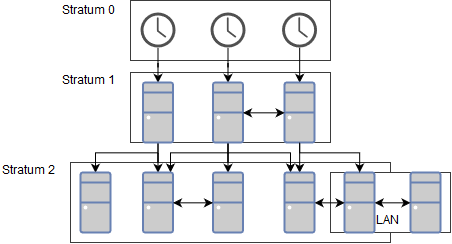
\includegraphics[scale=0.4]{synchronization/fig/NTP.png}
	\caption{An DFA that accepts any input that contains two '1' symbols in a row}
	\label{fig:NTP}
\end{figure}

\noindent Pros of network time protocol is that the client can be connected to more then one severer to get time, itis cheaper to develop NTP then PTP. Has feature called "Insane Time" which prevents synchronization witha server who is 1024 seconds apart.

\noindent Cons requires at lest one interface through wide area network which leads to security issues. Below stratum
15 devices are held unsynchronized.
Cons requires at lest one interface through wide area network which leads to security issues. Below stratum15 devices are held unsynchronized.
		\clearpage
\chapter{Real-Time Ethernet} \label{ch:realTimeEthernet}

Ethernet is a networking standard used in local area networks (LAN) that can a support a real-time system using packet switching, high bandwidth and low interference. We will look at the history of Ethernet and what challenges lay back then, a single segment Ethernet setup with CSMA/CD technology, then multi segment Ethernet with the spanning-tree protocol (STP) and a implementation of it.

\section{The history of Ethernet and single segment}

Ethernet was developed at Xerox PARC in 1973 and commercially introduced in 1980 as the so-called "DIX" (Digital, Intel, Xerox) standard with a bandwidth of 10Mbit/s, using coaxial cables and described as a technology for local-area networks". Ethernet became dominant over the likes of Token Ring and Token Bus in the end of the 1980's, because Ethernet was more adaptive than these proprietary protocols and quickly switched to the twisted-pair wiring (UTP, unshielded twisted pair), reducing cost, complexity and boosting transmission rates.

\noindent The Ethernet standard was intended for a typical office environment with workstations, but did also support PC-based controllers, PLC's and other devices, because it was an open-standard and easily accessible. Figure X illustrates a Plant-Control-Device environment, with higher response times at the plant level, more data transfers but less frequency.

\begin{figure}[h!]\label{}
	\centering
	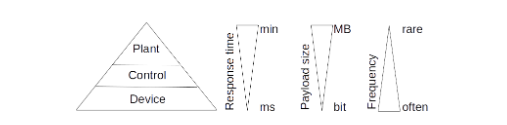
\includegraphics[scale=0.5]{realTimeEthernet/PlantControlDevice.png}
	\caption{The plant, control and device segments of a domain. Plant span entire facilities, control span plant floors and device span parts of plant floor.}
	\label{fig:plantcontroldevice}
\end{figure}

\noindent The first mid-80's Ethernet technologies (10BASE2, 10BASE5, and early 10BASE-T) constituted a so-called single segment network and relied on hubs, repeaters and the CSMA/CD (Carrier Sense Multiple Access with Collision Detection) protocol for sharing bandwidth on a shared medium. It was relatively low cost and flexible, but nondeterministic medium access made it hard to guarantee deadlines and use in a real-time system with no packet prioritization. Also speed was a function of the number of nodes on a network link. When sending, CSMA/CD implements carrier-sense by listening on the network for traffic. If it occurs, it does not transmit data. If no traffic for a certain period, it transmits data. Multiple Access allows more nodes to share the medium, but means collisions are more likely and that all packets are passed to all nodes. To mitigate this, the protocol brings Collision Detection, where a node listens for collisions on the medium, if they occur it sends a jam signal, back-offs for a random time period (exponential back-off algorithm) and tries again.

\noindent The truncated exponential back-off algorithm (EBA) retransmits after a random back-off time given by:

\[ T_{back-off}: r \times T_{slot} \]

\noindent with these properties:

\begin{itemize}
	\item $T_{slot}$ = $T_{dataout}$ + $T_{jam-back}$. The time it takes for the data to be sent to the point of collision and for the jam signal to get back. It is the max theoretical round-trip time.
	\item r $\sim$ \textit{u}[0, ..., 2\^{c} - 1], where \textit{u} is a uniform distribution.
	\item c is a local node counter, c $\in$ [1;$c_max$], and is reset after successful transmission. $c_max$ = 10 in the IEEE 802.3 CSMA/CD standard. Truncation means that after a certain number of increases, exponentiation stops and is reset.
\end{itemize}

\noindent For 10Mbit/s Ethernet, $T_{slot}$ = 51.2$\mu$s and decreases when transmission rates $\longrightarrow$ $\propto$. Figure \ref{fig:csmacd} shows how a collision on the wire, how the two re-transmissions collide and the random back-off timer in effect.

\begin{figure}[h!]\label{}
	\centering
	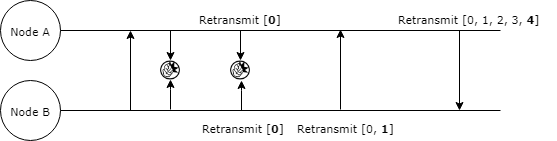
\includegraphics[scale=0.5]{realTimeEthernet/CSMACD.png}
	\caption{CSMA/CD in effect with random re-transmissions upon collisions.}
	\label{fig:csmacd}
\end{figure}

\noindent A conceivable drawback of the back-off algorithm is that it can introduce medium monopolization by one node in a network, $Node_{a}$, depriving another node, $Node_{b}$ of time to send. As the back-off algorithm is random, if $Node_{a}$ is more successful than $Node_{b}$ at sending packets, $Node_{b}$'s collision counter might increase beyond that of $Node_{a}$, resulting in exponential wait times for $Node_{b}$. In the next chapter we look at how to solve collisions using network segmentation.



\section{Multi-segment Ethernet and STP}
\subsection{Multi-segment}

To solve issues with collisions it is neccessary to split the network into different domains each with their own collision domains. This was made possible with the introduction of switches which segmented the network on the Link layer (OSI Level 2) in 1990 by Kalpana, which was later acquired by Cisco. The segmentation resulted in traffic no longer being broadcast across multiple nodes, and at the extreme each node is connected directly to a network switch forming a micro segment. In 1998 full 8 wire twisted pair wires were introduced which allowed for Pysical layer (OSI Level 1) segmentation as the cables were now full duplex. In the years since the price of CAT 5 cables and switches has dropped, and eventually the older technologies were phased out in most networks, removing all potential for collisions. To ensureAs a consequence of the collision free networks it became possible to exceed 10 Mbps and modern networking cards support 100 Mbps at a minimum and 1 Gbps is becoming more common. To insure thees network speeds there was made spanning-tree protocol (STP) which is building for making forwarding topology free-loop and for reducing broadcast radiation. 

\subsection{Spanning-tree protocol}
The idea behind the STP protocol is to have only one way from one node to another one. As in the Figure \ref{fig:STP} A is before the algorithm B is after the algorithm. The STP finds the fastest and loop-free path between two nodes.

Kruskal's algorithm:

\begin{enumerate}
	\item Sort the edges by weight, increasing, and add them to a list.
	\item Add the edge with the lowest weight from the list and remove it from the list hereafter.	
	\item Add the next edge with the lowest weight if adding the edge does not create a circle and remove it from the list hereafter.
	\item Repeat 4 step until a minimum spanning tree has been formed.
\end{enumerate}

The algorithm was made during the course using networkx library in python the Figure\ref{fig:STP} shows graphical example for our implementation of Kruskal's algorithm.

\begin{figure}[H]\label{}
	\centering
	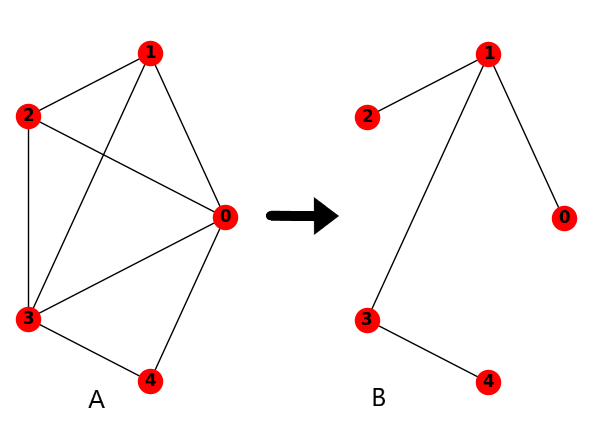
\includegraphics[scale=0.5]{realTimeEthernet/Image/STP.png}
	\caption{Spanning-tree protocol exercise}
	\label{fig:STP}
\end{figure}


\section{Multi-segment real-time Ethernet}

%Maybe put this together with multiSegmentStp?

To solve issues with collisions it is neccessary to split the network into different domains each with their own collision domains. This was made possible with the introduction of switches which segmented the network on the Link layer (OSI Level 2) in 1990 by Kalpana, which was later acquired by Cisco. The segmentation resulted in traffic no longer being broadcast across multiple nodes, and at the extreme each node is connected directly to a network switch forming a micro segment. In <Year> full 8 wire twisted pair wires were introduced which allowed for Pysical layer (OSI Level 1) segmentation as the cables were now full duplex. In the years since the price of CAT 5 cables and switches has dropped, and eventually the older technologies were phased out in most networks, removing all potential for collisions. As a consequence of the collision free networks it became possible to exceed 10 Mbps and modern networking cards support 100 Mbps at a minimum and 1 Gbps is becoming more common.

\subsection{Store and forward vs. Cut through}

Switches have two modes of operation, 'store and forward' mode or 'cut through' mode. Both modes have their own advantages and disadvantages with neither being objectively better. 

* Store and forward: In this mode the switch stores each package and verifies that it has been received correctly. If the package has been corrupted then the switch will request a retransmission from the previous node. This mode minimizes the transmission of corrupted packages, reducing the overall congestion in the network and improving the performance in a high noise environment. The downsides are that this mode is resource intensive from the switch which increases latency and throughput, especially when there is much traffic on the network.
* Cut through: In this mode the switch starts sending the package as soon as it starts receiving it, reducing latency and saving resources for data transmissions. This reduction in latency (down to 10 ms between two nodes) makes Cut through more suitable to real time systems. The downsides of cut through switching is that corrupted packages will also be transmitted along with other traffic allowing corrupt data to get further through the network before being caught and retransmitted. 

Many switches have the ability to switch between store and forward and cut through modes depending on the context.

A major challenge for switches is the need to manage routing of messages to the correct recievers, preferably without being manually configured to do so. The switch will manage a list of MAC addresses reachable from each port by monitoring the sender addresses of incoming packages. When in doubt the switch will simply broadcast the message to all active ports aside from the sender. Due to these broadcasts there is a risk of the network flooding itself in cases where 

		\clearpage
\chapter{Middleware} \label{ch:middleware}					\clearpage
\chapter{Consistency} \label{ch:consistency}

Consistency is a condition where all nodes in a system agree on the current state of the system and see the same data at the same time. In a centralized system, this challenge often becomes more manageable, as decisions that change the state of the system are stored in shared memory between processes. In a distributed system with multiple nodes, each processor has its own private memory and the ability to change the state of the system, so state information must be passed from one node to the next. This can create consistency problems, when nodes become out of sync or somehow do not reflect the current state of the system due to server failures, bandwidth bottlenecks or network topology changes. In this chapter we look at the CAP and PACELC theorems for consistency and replication, and discuss various consistency models used in distributed systems.

\section{The CAP theorem}
The CAP stands for Consistency, Availability and Partition Tolerance, and these are three attributes of a distributed system. The consistency attribute means that if a node has been written to, then if another node is read from, it will return what was just written to the other node. In other terms, if a node is written to it will return the newest version of the data given to any node in the system. The availability attribute promise that when a node is spoken to it will respond, unless that node has failed, the availability attribute allows for failed nodes but in any other case it will respond. The partition tolerance means that when the network is partitioned then whatever other promises are made about the system, it will still keep those promises. A network is partitioned, when messages can't flow from one machine to another. This might happen if you have two different data centers and the connection between the two is separated. On Figure \ref{fig:cap_triangle} a simplified version of the theorem can be seen, as well as examples of which attributes, some  of the more known databases, support.

\begin{figure}[h!]
	\centering
	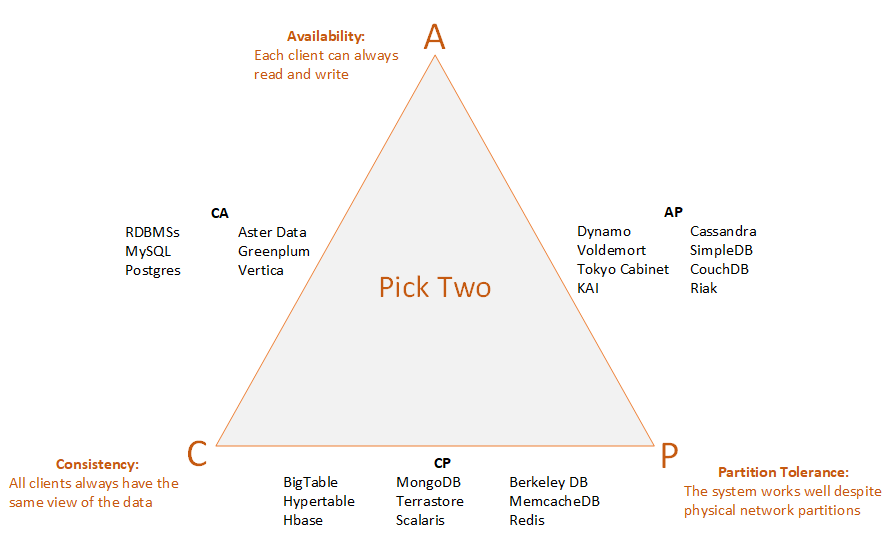
\includegraphics[width=0.61\linewidth]{consistency/fig/cap_triangle.png}
	\caption{CAP theorem triangle, with examples of database attribute support.}
	\label{fig:cap_triangle}
\end{figure}

The CAP theorem says, that a distributed system, can only have up to two of these attributes fulfilled at a given time. On Figure \ref{fig:cap_proof} the proof, of the three scenarios, is illustrated. Case A; there is a partition between Node A and Node B. The new data that is send to Node A can not be read from Node B, therefor the system is not consistent. Case B; there is a partition between Node A and Node B. Since the new data can not be send between the nodes and the system won't send old data Node B won't respond to the read request, this makes the system not available. Case C; there is no partition between the nodes, therefor the system is not partition tolerant.

\begin{figure}[h!]
	\centering
	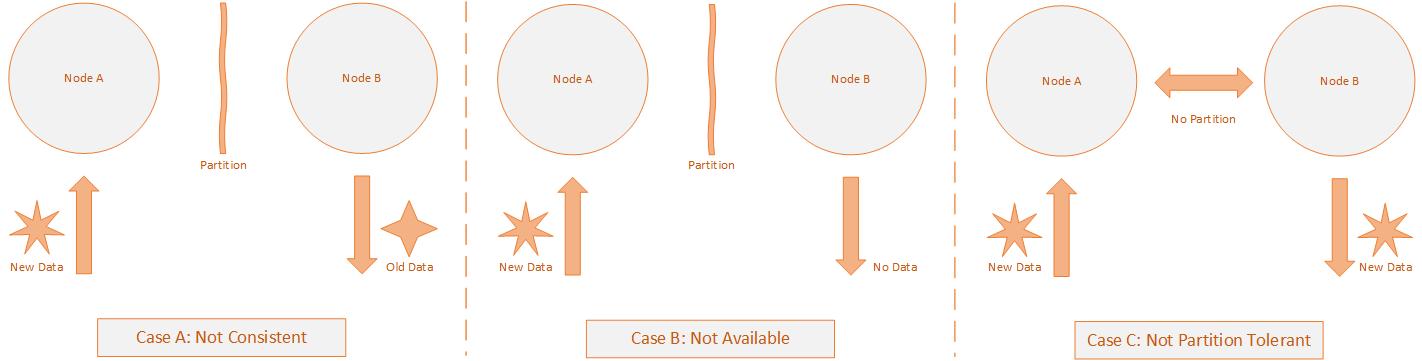
\includegraphics[width=0.9\linewidth]{consistency/fig/cap_proof.png}
	\caption{CAP theorem three possible outcomes.}
	\label{fig:cap_proof}
\end{figure}


\section{PACELC}
The PACELC theorem is a addition to the CAP theorem. This addition tries to describe a more full picture where that even in the absence of partitions there's a tradeoff between consistency and latency. In CAP, one must choose between high availability and consistency. This leaves no option for mission-critical applications but to sacrifice consistency because high availability is a given. This logic is not right because the P in CAP is a mix of \textit{partition tolerance} and a \textit{actual network partition}. Therefore it is wrong to assume the systems that reduce consistency in the absence of any partitions are doing it because of CAP. PACELC handles the cases when a network partition have or not happened.

\noindent The theorem states: If there is a partition \textbf{P}, how does the system trade off availability \textbf{A} and consistency \textbf{C}. Else, when the system is running normally in
the absence of partitions, how does the system trade off latency \textbf{L}
and consistency \textbf{C}\footnote{Appendix 1 - Fischer\_DIPS\_S05\_Synchronization\_Slides, p.~13}

\noindent Apache's \textbf{Cassandra} database system is a PA/EL system. If a partition happens, it will give up consistency for availability, and during normal operation gives up consistency for lower latency. Google's \textbf{BigTable}
follows ACID\footnote{ACID (Atomicity, Consistency, Isolation, Durability) is a set of properties of database transactions intended to guarantee validity even in the event of errors, power failures, etc.} hence PC/EC. It will refuse to give up consistency and pay the price in terms availability and latency costs to achieve it. \textbf{MongoDB} can be classified as a PA/EC system. In the default configuration, the system guarantees reads and writes to be consistent.\footnote{\cite[p.~42]{Abadi2012}}
When a system have a network partition happen to it there is a few options for replication the data.
\begin{enumerate}
	
	\item Data updates sent to all replicas at the same time.
	\begin{enumerate}
		\item Using a preprocessing layer gives us consistency but increased latency.
		\item Not using a preprocessing layer will decrease latency but can only offer eventual consistency.
	\end{enumerate}
	\item Data updates sent to an agreed-upon location first
	\begin{enumerate}
		\item Synchronous the master node waits until updates made it to the replicas. Therefor gaining consistency but pays latency.
		\item Asynchronous treats the update as if it were completed before being sent to a replica.
	\end{enumerate}
	\item Data updates sent to an arbitrary location first.
		\begin{enumerate}
		\item Synchronous then the latency problems of (2)(a) are present.
		\item Asynchronous consistency problems same as (1) and (2)(b) are present.
	\end{enumerate}
\end{enumerate}

\begin{table}[H]
	\centering
\begin{tabular}{|c|c|c|c|c|}
	\hline 
	System & A & C & L & C \\ 
	\hline 
	Cassandra & X &  & X &  \\ 
	\hline 
	BigTable &  & X &  & X \\ 
	\hline 
	MongoDB &  & X & X &  \\ 
	\hline 
\end{tabular}
  \caption{This is my one big table} \label{tab:PACELC}
\end{table}

\newpage
\section{Consistency models}

Consistency models are used in distributed systems like shared memory storage, filesystems and databases to amend the issues that distributed write and read access could have to such a system. A consistency model define a given set of rules a operation must follow when accessing the data and can be seen as a contract between a running process (the programmer) and the system. If the process comply with this contract, then memory will be consistent and the output of reading, writing, or updating the memory will be predictable. For example in relational database systems, transactions abide by the ACID principle, where consistency ensures that any transition will bring the database from one valid state to the next and that data should follow a set of rules. Assume a relational database in a cluster that contain row $R_x$ and that this row is replicated to nodes $Node_a$ and $Node_b$. A client $C_i$ then writes $R_x$ on $Node_a$. Subsequently another client $C_j$ reads $R_i$ from $Node_b$. A consistency model has to determine if $C_j$ sees the write from $C_i$ or not.

\noindent Consistency models can be classified as strong or weak. A strong consistency model guarantees that the order and visibility of updates are equivalent to that of a centralized (non-replicated) system with only one process, that is updates are immediately replicated to all nodes. A weak consistency model does not make this guarantee. We will now look at both strong and weak models and consider them for a distributed system:

\noindent \textbf{Linearizability}: A strong consistency model that ensures that all operations appear to have run atomically (in isolation, independent from concurrent processes) in an order that is consistent with the global real-time ordering of operations. If a distributed database follows this model, than it would appear centralized to its clients. No matter how clients execute operations, the result would be the same as if they we executed in some sequential order and these operations appear in their order of executing.

\noindent \textbf{Sequential consistency}: A strong consistency model that mimics the linearizability one, but does not require that two independent operations from different clients respect the real-time ordering of operations in a system. With this model, operations can be re-ordered as long as each node observe the ordering consistently. A benefit of the two strong consistency models is that a client or programmer can replace a centralized system with a distributed one without facing data consistency issues.

\noindent \textbf{Client-centric consistency:} A range of various weak consistency models that makes guarantee to clients (users) of data. It ensures that a client may never see old versions of data, if they have already seen a newer one. This can be implemented with client-side caching, so if the client suddenly connects to a node with old data on it, then the application will present a cached version to the client. Still this may not be the newest version of the data globally, hence the weak consistency predicate.

%%http://www.bailis.org/blog/safety-and-liveness-eventual-consistency-is-not-safe/
%%https://www.allthingsdistributed.com/2008/12/eventually_consistent.html
\noindent \textbf{Eventual consistency}: A weak consistency model that guarantees that if an update has changed the state of one node in a system, after a undefined amount of time all nodes will reflect the same state, if no more values are changed. During this period of time (the inconsistency window) some nodes may be consistent and some may not. The size of this window is determined based on communication delay between nodes, system load and the number of nodes involved in the replication scheme. DNS (Domain Name System) and popular NoSQL datastores like Cassandra and DynamoDB implement a eventual consistency model. Eventual consistency is often refereed to as a liveness property, whereas a stronger model like linearizability is a safety property.

\noindent \textbf{Casual consistency}: A weak consistency model that captures the causal relationships between operations in the system, meaning that an update on a process becomes visible to another process only it has relationship with that process. If the operation on a process $P_i$ influences another write operation on process $P_j$, then these two operations are causally related. After updating $P_i$, it communicates to $P_j$ that a value was updated, and subsequent access by $P_j$ will return the updated value and writes will supersede it.

\noindent To recap, which model you choose is a tradeoff between availability and consistency. A system with high avaliabily may suffer from weak consistency and wise versa. We saw this in the PACELC theorem.				\clearpage
\chapter{Fault tolerance and consensus} \label{ch:faultToleranceandconsensus}

In a distributed system there is a need for nodes to automatically recover from technical failures or partitions. If a node fails, the rest of the system should continue to operate without disturbing the clients. This is called fault tolerance. When the node has been repaired, it should be able to rejoin the distributed system and have its state brought up-to-date with the rest of the nodes. We say that a system is in a consensual state when a majority of nodes have agreed on some final value. In this chapter we look at the topic of fault tolerance and how it can be archived using the Raft consensus algorithm in a distributed system.

\section{The basics of fault tolerance}

A major difference between centralized and distributed systems is that we can experience partial failures in a distributed one. Suddenly, nodes can malfunction or become inaccessible due to network partitions. This can lead to decreased usability for clients. Therefore a strategy needs to be in place that can handle these kinds of failures. Without such the decrease of the operating quality for users would be proportional to the seriousness of the failure. Before diving into what types of failures we may witness, it is important to understand what values we seek in a distributed system and how they differ from each-other.

\noindent \textbf{Availability}: Availability is the quality of being able to be used right away. It is defined as a probability that the system will be ready when users need it to be. For high-availability or mission-critical systems, we usually see an uptime around five nines, which means the system has a probability of 99.999\% to be ready when users call.

\noindent \textbf{Reliability}: Reliability is the quality of being trustworthy and be able to produce consistency in measurements, i.e. the system will run without failures. It is defined as a time interval instead of a instance in time. If a system has high availability but still crashes randomly at times, it is unreliable. If a system never crashes, but is often shut down due to maintenance at a specific time, it is reliable.

\noindent \textbf{Safety}: To archive safety in a system, nothing fatal can happen should the system experience a failure. We often see this in mission-critical systems, where even a brief outage can have severe consequences. This could be a space rocket or a power plant facility. In less crucial systems, safety may not play such a huge role.

\noindent \textbf{Maintainability}: Maintainability tells us how easy a failed system can be examined, repaired and have worn-out components replaced by newer ones. We often see a correlation between high maintainability and high availability. 

\noindent \textbf{Atomicity}: Finally, atomicity is the quality of a operation or transaction that is indivisible and irreducible. Either it completes fully or nothing happens at all. This correlates to safety and can be seen especially in banking systems, where a money transaction between two accounts often involves multiple system and must be reversible should something interfere.

\noindent A system is said to fail when it cannot meet its promises or is unable to perform its required function. Failures are sometimes caused by errors, but they do not have to lead to failures, however. The cause of an error is a fault, that is an incorrect step, process or definition in a software application which causes the system to perform in an unintended manner. An technical fault in a branch of code on a node could lead to it experiencing an error, which could make it crash during execution. If other parts of the system depend on this node, the error could lead to a system failures. To classify these we use the following terms:

\noindent \textbf{Crash failures} occur when a node suddenly halts, but was working fine up until that point. A physical action must be taken to bring the node back up. \textbf{Omission failures} occur when a node does not respond to a incoming request. The request can malformed or perhaps the node fail to generate a response. \textbf{Timing failures} happen when a node does not respond within a time limit, maybe due to network delay or excessive load. \textbf{Response failures} is when a node respond, but its response is incorrect or is out of step with the current state of the system. \textbf{Arbitrary failures} are random and can occur at any time. These can be hard to narrow-down and correct.

\noindent To gain fault tolerance in a distributed system, we should seek to mask the occurrence of failures from other processes and have a back-up plan ready (redundant nodes) in case they should happen. We should also implement self-stabilization, so that the system will converge towards a correct state, no matter the initial one. Consensus is the key to archive this.

\section{The Raft consensus algorithm}

			\clearpage
\chapter{Leader Election} \label{ch:leaderElection}

A leader performs sort of the conductor role in a distributed system and is responsible for maintaining consensus. Putting this task on one job has the benefit of avoiding synchronization conflicts when individual nodes has to update their state, but also ensures consistency in the process and provides safety as well. Ideally, the nodes should not know each-other and send commands among them, but solely relay on the leader telling them what to compute. Therefore the task of selecting the leader becomes crucial. In this chapter we will look two popular algorithms to do so, the Bully and the ring algorithm, and then discuss other ways to elect the most appropriate leader.

\section{The bully and ring algorithm}

The algorithm was proposed by Garcia-Molina in 1982 and simply put elects the node with the highest id out of \textit{N} nodes with unique ids, hence the name. The current leader would be the one with the highest id at time \textit{t} in a star network cluster. When any node $N_i$ notices that the leader is not responding, it starts an election as follows:

\noindent Node $n_i$ sends a ELECTION message to all nodes with higher ids, that is $n_i+1, n_i+2 ... n-1$ nodes. If it does not hear from any, node $n_i$ wins the election. If any node with a higher id responds, it will take of the election process and $n_i$ will not contribute further. During this process our node $n_i$ can receive a ELECTION message from a node with a smaller id. It will acknowledge the message and begin a new election, if one is not already taking place. This continues until basically \textit{N-1} has given up, leaving the last node as the new leader or coordinator. The node will put a message to all other nodes announcing its leadership. If a node with a higher id is added to the cluster, it will take the reins the conduct a new election, which it will win.

\noindent The benefits of this algorithm is clearly is intuitiveness, simplicity and its fairly low amount of traffic generated to elect a leader, but may lack a more sophistic approach to it if the node with the highest id is unreliable or unstable. One could imagine the leader quickly becoming overloaded with leader obligations, such as replicating a data log to \textit{N} nodes and serving clients, which would simply trigger a whole new election.

\noindent The ring algorithm works similarly to the bully, but has nodes in a logical ring topology rather than a star. Each node knowns its successor. If a node does not receive a sign of life from the leader, it starts an election by sending an ELECTION message containing its id to its successor. The successor adds its id to the message and forwards it. This continues for \textit{N-1} nodes until the messages gets back to the initiating node, which then sends out a COORDINATOR messages informing nodes of who the leader is (the one with the highest id) and which nodes are part of the ring.

\section{Other ways to choose a leader}

One shortcoming of the bully algorithm is its naive approach to selecting a leader, where it simply picks the node or process with the highest id. You could design your system such as the node with the most resources or raw CPU power also had the highest id, and as you go down in identifiers the resources available drops, but that is not always possible or convenient. Let us address two few factors that could be more profitable including in the election process:

\noindent \textbf{Computational resources}: Obviously, the leader has to do more than everybody else, so measuring its computational capabilities before casting ones ballot could be advantageous. Things like CPU power, memory, available storage for replication logs and battery power left if we are in a wireless setting spring to mind.

\noindent \textbf{Server or network load}: A distributed system operates a varying work loads and network resources may come and go. During day time, the server handling orders at a web shop may be more stressed taking customer orders than at night, which could make it less applicable as a leader. Also data traffic congestion at a certain node could play a role as well.

\noindent There is no silver bullet when selecting the right leader election protocol, so application, system size and resources need to be considered. A small embedded system might be fine off with the bully algorithm, while a bigger and more complex system might need something else.			\clearpage
\chapter{Positioning} \label{ch:positioning}
This chapter is about location. We will cover absolute positioning meaning independent and not relative to something else. Relative on the other hand is in relation to something else. A hybrid solution is a mix of both
\section{Absolute positioning}
\section{Relative positioning}

A relative position is a position that is relative to something absolute. A technique called dead reckoning is very useful in situations where one have to move away from a absolute position, therefore will not be able to get another for a while. Such as in a network game or outside hiking with no Global Positioning System (GPS). To use dead reckoning you need to keep track of things that can help you navigate, such as:

\begin{itemize}
\item Direction of travel.
\item Pace.
\item Time of walking.
\item Landmarks.
\end{itemize}

When our hiking trip starts, we know we are at a absolute position, that is our base camp, and we want to reach the destination as shown in figure \ref{fig:deadrecdrawing}. We use our pace, compass and the landmarks to navigate to the destination.

\begin{figure}[H]
	\centering
	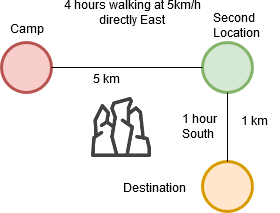
\includegraphics[width=0.4\linewidth]{positioning/positioning/deadRecDrawing}
	\caption{A hiking trip with navigation using dead reckoning.}
	\label{fig:deadrecdrawing}
\end{figure}

But dead reckoning suffers from errors that are cumulative, for example, if the first part of the trip had ended up being 8 kilometers instead of 5 then even if the second part goes according to plan, you are still going to end up in the wrong place. A way to solve this problem is to find your absolute location with bearings from time to time as that will reset the drift in regard to possible errors.

\section{Dead recking in network games}

Dead recking is not only used at sea or to navigate at land, but also in distributed virtual environments. When people across the planet play network games, they are sometimes located very far from each other, geographically. Pantel and Wolf\footnote{\cite{Pantel2002}} explores different dead reckoning schemes in various games such as sports and action games. They measured eight prediction schemes: Four predictions of positions, three predictions of input and one with no prediction. As shown in Figure \ref{fig:wolfpeperimage} Prediction 1 which predicts the position by assuming a constant velocity yields the best result.

\begin{figure}[H]
	\centering
	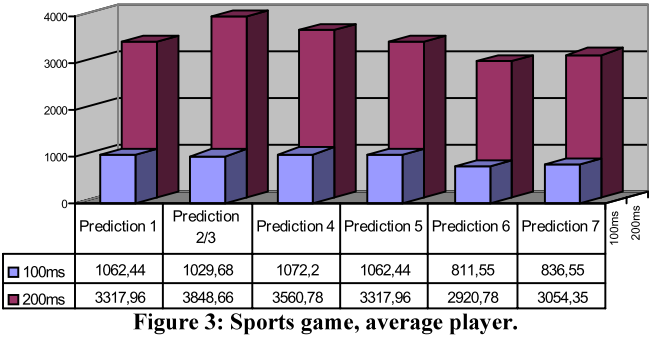
\includegraphics[width=0.5\linewidth]{positioning/positioning/wolfpeperImage}
	\caption{Prediction 1 was best in a sports game}
	\label{fig:wolfpeperimage}
\end{figure}

The article concludes that the different schemes tested upon were useful for network games, but could not reduce the latency directly, the impact, on the game, could be reduced however.
\section{Hybrid positioning}

The absolute positioning method is quit accurate but still it suffers from noise. On the other hand relative position has a lot uncertainty, because of the physical interference. By combing these two positioning methods we can get more precise location based on sensor measurements from absolute and prediction from the relative positions. This combination is called hybrid positioning. One of the methods achieving hybrid position is with Kalman filter, which will be described below.

\subsection{Kalman filter}

The Kalman filter was made by Rudolf E. Kalman. It was developed for Apollo mission to the moon, to track the location of the space shuttle. This method is still used, because it dos not require a lot of processing power and memory space. The reasoning is that the method dos not need to save any data apart the model of movement and and previews position.

The process of the filter is as follow:
\begin{enumerate}
	\item Predict the position form previews position and movement of the model
	\item Correct the position with the measured data
	\item Repeat step 1 and 2
\end{enumerate}

Fidure\ref{fig:KalmanfilterRotation} shows it visually.

\begin{figure}[H]
	\centering
	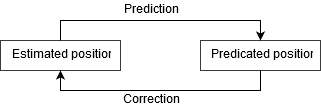
\includegraphics[width=0.4\linewidth]{positioning/positioning/KalmanFilterProcess}
	\caption{Kalmans filter principal}
	\label{fig:KalmanfilterRotation}
\end{figure}

In the Figure\ref{fig:Kalmanfilter} is displayed two case how the filter works. First one is when time(T-1) and time(T). In this case the filter goes closer to the measurement Gaussian, because it is more reliable.The hybrid position probability is higher then absolute and relative positioning this is because the absolute and relative position Gaussian's are multiplied together. The second case is in the period (T) and (T+1) in this case the measurements has a lot more noise in them. Then the estimation is moving further from the measurement Gaussian, because of the lower probability. 

\begin{figure}[H]
	\centering
	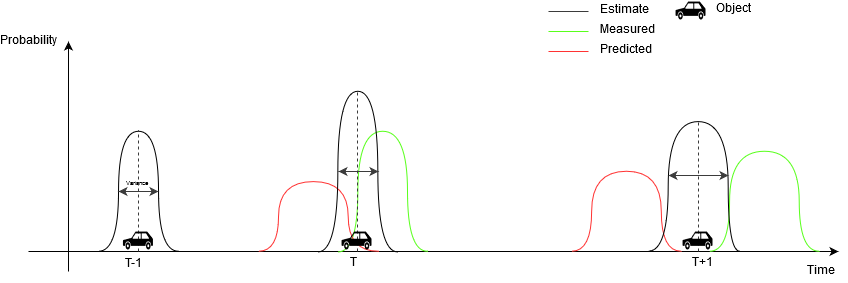
\includegraphics[width=0.7\linewidth]{positioning/positioning/DiagramKalman}
	\caption{Kalmans filter example}
	\label{fig:Kalmanfilter}
\end{figure}

%\section{Hybrid positioning and Kalman filter}
%The absolute positioning method is quit accurate but still suffers from noise. On the other hand relative positioning has a lot of uncertainty, because of the physical interference. By combing these two positioning methods we can get more precise location based on sensor measurements from absolute and prediction from the relative positions. This combination is called hybrid positioning. One of the methods achieving hybrid position is with Kalman filter.
%The Kalman filter was made by Rudolf E. Kalman and developed for the Apollo 11 mission\footnote{\cite{Grewal2010}} to the moon to track the location of the space shuttle. This method is still used because it does not require a lot of processing power or memory space. The reasoning is that the method does not need to save any data apart from the model of movement and the previous position. The filter predicts a position based on the model and previous positions. After the prediction, the real position is being measured and the filter corrects its prediction by multiplying both Gaussian distributions thus producing a more precise prediction of position.
%In figure \ref{fig:Kalmanfilter} we see how the filter is working. There are two cases in it. First one is when time is (T-1) and (T). In this first case we can see that the filter goes closer to the measured distribution, because it is more reliable. Also from the graph we can see the power of hybrid position: The probability is estimating the position correct is higher than absolute and relative positioning. The second case is when time is (T) and (T+1). In this case the measurements contain a lot more noise. Then the estimation is moving further from the measured distribution because of the lower probability.
%The Kalman filter was made by Rudolf E. Kalman. It was developed for Apollo mission to the moon, to track the location of the space shuttle. This method is still used, because it dos not require a lot of processing power and memory space. The reasoning is that the method dos not need to save any data apart the model of movement and and previews position.
%In the Figure\ref{fig:Kalmanfilter} is displayed two case how the filter works. First one is when time(T-1) and time(T). In this case the filter goes closer to the measurement Gaussian, because it is more reliable.The hybrid position probability is higher then absolute and relative positioning this is because the absolute and relative position Gaussian's are multiplied together. The second case is in the period (T) and (T+1) in this case the measurements has a lot more noise in them. Then the estimation is moving further from the measurement Gaussian, because of the lower probability.
				\clearpage
\chapter{Discussion} \label{ch:discussion}

Key points:

We have learned various techniques that can be applied to the development of distributed systems to both enable us to provide .... various good stuffs.

Of particular interest to the authors were the technologies surrounding the topics of ...?

Why did we do this?
				    \clearpage



\chapter{Conclusion} \label{ch:conclussion}
Throughout this report we have discussed various methods for implementing distributed systems in stable and scalable ways. We have discussed the concept of time-synchronization through different clock-types and how they can be applied to maintain timelines between different applications. Real-time distribution in the system can be achieved, once there is consensus on time domain. Other problems can occur however and we discussed the concepts of consistency, fault tolerance and consensus, which give us much needed stability by eliminating many of the fragile factors from the architecture of the distributed system.

Middleware has been an economic driver for the growth of distributed systems in recent years, by simplifying development of new systems, by abstracting away the complexities of dealing with system distribution.

Positioning shows us methods for exploring physical and virtual worlds, and integrating our systems into them. Location and tracking have been of special interest due to their applications in various fields.

%Key points:
%	How have we approached bypassing the limitations imposed by the laws presented in the introduction
%	Surprising discoveries from the class?
%	The collective effort of devices is greater than the sum of their parts.
%	Computers will always need more processing power and distributed systems are a potential method for gaining additional processing power at low cost.				    \clearpage
\chapter{Perspectives} \label{ch:perspectives}				\clearpage
\bibliographystyle{plainnat}
\bibliography{bibliography/mendeley/DistributedAndPervasiveSystems} \label{ch:bibliography}

%TODO: Insert ref.
%%http://www.drdobbs.com/jvm/what-is-priority-inversion-and-how-do-yo/230600008				\clearpage

%etc...

\end{document}